\chapter{The~\texttt{porthos2}:~implementation}
\label{ch:impl}

The main reason for commencing the work on \porthos[2] was the need for processing real-world C programs, which, at first, requires the input language to be extended.
This implies the support not only for new syntactic structures of C language (such as the \texttt{switch} statement or the postfix increment operator \texttt{i++}), but also for its fundamental concepts and features (such as types, pointer arithmetic or first-order functions), which requires revision of the whole architecture of the tool.
Although far not the entire C language has been supported (that, considering its complexity and numerous pitfalls, goes far beyond current thesis%
\footnote{To ensure that, we have merely to look at existing C compilers, for instance, the open-source \texttt{gcc} compiler, that uses a C parser written in more than 18.5 thousand lines (see \url{https://github.com/gcc-mirror/gcc/blob/master/gcc/c/c-parser.c})}%
), we consider the accomplished work as a step towards this.
%This applies not only to instances that simply constitute the syntactic sugar of C language (such as the \texttt{switch} statement or the prefix increment operator \texttt{++i}), but also to its fundamental concepts and features (such as pointer arithmetic or structures).
%However, the architecture of current version of \porthos{} does not allow to ... as it is ....
% Although and optimisation of the tool so that it is able to process real C programs in perspective.

%In current Chapter we discuss the new architecture of \porthos[2].

% function invocations/calls: inlining with binding
% contexts: for now, no ctxs
% comparing to cprover (https://www.cprover.org/cbmc/doc/manual.pdf, page 45, absatz about 'goto') where "the loop is unwound a given number of times" , we SHOULD have 2 modes of unrolling: 1) number of times, and 2) number of high-level instructions executed
% TODO(code): (https://www.cprover.org/cbmc/doc/manual.pdf, page 45) "The break and continue statements are replaced by equivalent goto statements as described in the ANSI-C standard."

% TODO: arrays: cprover manual page 48


%\section{The architecture of \porthos[1]}
\section{General principles}
\label{ch:impl:principles}

The existing implementation of \porthos[1] does not distinguish the event-based program model from the high-level AST, they both are encoded into single SMT-formula (see classes of package `\texttt{dartagnan.program}' of \porthos tool).
Moreover, the syntax tree was implemented as a mutable data structure, which is being modified at all stages of the program (for instance, see the methods `\texttt{dartagnan.program.Program.compile(...)}' of \porthos{} that recursively compute some properties of the AST and change its state).
We are inclined to consider this architecture as one that is fast to develop, but hard to maintain (since it is difficult to guarantee the correctness of the program) and extend (since adding the support for a new high-level instruction requires changing multiple components of the program, from parser to encoder).
%Moreover, we encounter serious problems when we need to add support for control-flow jumps (as \texttt{continue}, \texttt{break}, \texttt{goto} in C).

% todo: in old porthos the strategy soft: print info about error. new: exception on any detected violation of any invariant

Therefore, while working on the new design of \porthos[2], we decided to clearly separate the high-level intermediate code representation (implemented as a recursive AST structure) from low-level event-based representation (implemented as an event-flow graph).
Such a modular architecture allows to support multiple input languages by parsing them and converting parsed syntax trees to a simplified AST. which, along with all other data-transfer objects (DTO), must be immutable, so that it is possible to guarantee the correctness of the program by controlling its invariants.
The immutability in \porthos[2] is implemented via \texttt{final} fields that are assigned by the immutable-object values (either a primitive type, or another immutable object, or an immutable collection provided by the library Guava by Google%
\footnote{Guava project repository: \url{https://github.com/google/guava/}}%
).

During the development of \porthos[2] we mainly followed the \textit{KISS~principle}, which can be exhaustively described in 17 Unix Rules of Eric Raymond~\cite{raymond2003art}.% which include the rule of modularity, the rule of clarity, transparency, extensibility, etc.
The following list summarises the main rules we followed during the development of \porthos[2]:

\vspace{0.5em}
\begin{enumerate}[nolistsep]
  \item \textit{Robustness:}
    \begin{enumerate}[label*=\arabic*.]
      \item usage of immutable data structures for all DTOs;
      \item interrupting the work on errors;
      \item modular architecture: each module can be tested independently;
      \item usage of software design patterns if necessary;
    \end{enumerate}
  \item \textit{Transparency:}
    \begin{enumerate}[label*=\arabic*.]
      \item following the principles of simplicity and readability;
      \item clear and informative program output;
    \end{enumerate}
  \item \textit{Efficiency:}
    \begin{enumerate}[label*=\arabic*.]%[leftmargin=1.5em]
      \item keeping the trade-off between execution time and memory usage;
    \end{enumerate}
  \item \textit{Extensibility:}
    \begin{enumerate}[label*=\arabic*.]%[leftmargin=1em]
      \item clear modular architecture.
    \end{enumerate}
\end{enumerate}


As \porthos[1], the \porthos[2] uses the open-source SMT solver \texttt{Z3} from Microsoft Research~\cite{de2008z3}. However, unlikely its predecessor, the \porthos[2] has an additional abstraction level \zformula{} (see Section~\ref{ch:impl:model:zformula}) that allow to use any other SMT solver. %TODO: *should* allow?

The programming language choice for \porthos[2] was also made in favour of \textit{java}, firstly, in order to be able to reuse some parts and concepts of \porthos[1] that is written in java, and secondly, because the authors find the object-oriented (OOP) concepts of java suitable for modelling languages.
Although java does not show best results in performance benchmarks (for example, comparing to C++~\cite{hundt2011loop, oaks2014java}), the performance cornerstone of \porthos[2] (as well as any other SMT-based code analyser) is the phase of solving the SMT-formula, which is left to the third-party SMT-solver \textit{Z3}%
\footnote{The Z3 project repository: \url{https://github.com/Z3Prover/z3}} %
invoked from \porthos[2] via java API.
However, considering the perspective of using \porthos[2] as a static analyser for real-world programs, the memory optimisation problem must also be taken into account during both encoding and solving stages.
It is worth noting that, for the reasons of simplicity, the \porthos[2] is not a concurrent program, however, we believe that, due to its modular architecture, it can be easily parallelised on the level of program modules.


\section{Architecture}
\label{ch:impl:arch}

The general architecture scheme of \porthos[2] is presented in Figure~\ref{fig:arch}. On the picture, rectangles denote processing units (marked with gear sign with a unique number of the component).

\begin{figure}%[H]
    \centering
  %draft=true
  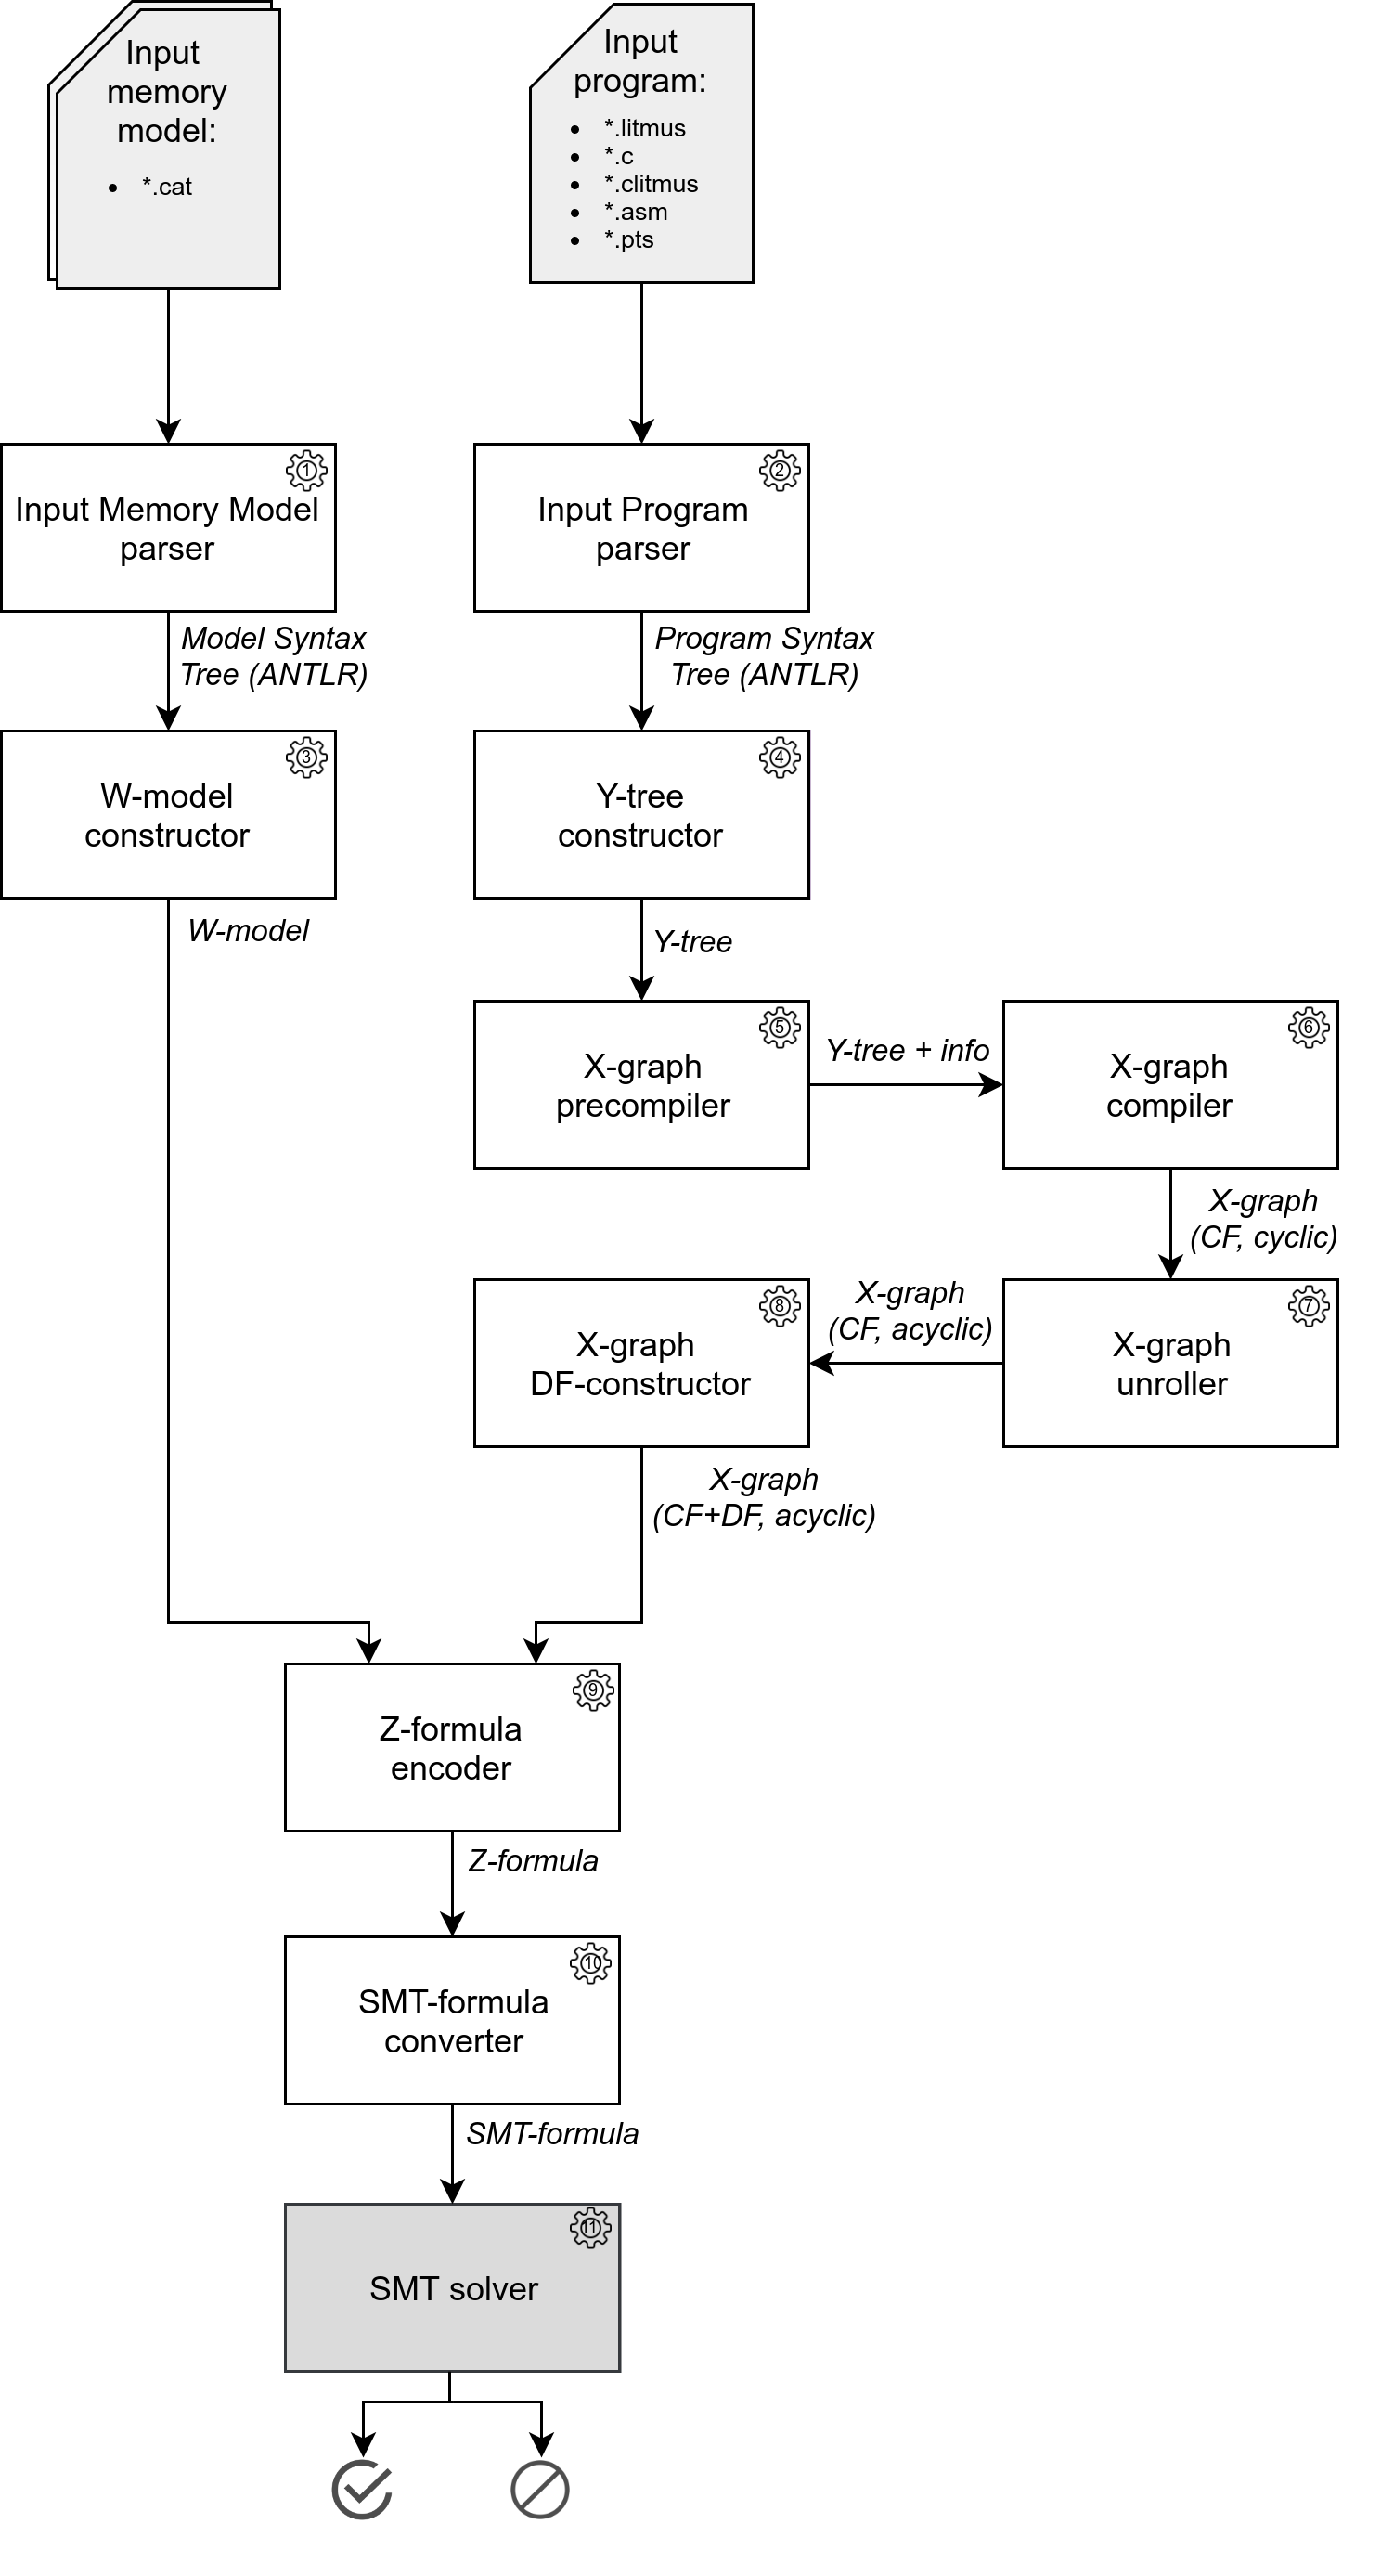
\includegraphics[height=.99\textheight,keepaspectratio]{img/my/draw.io/general_arch.png}
  \caption{The general architecture of \porthos[2]}
  \label{fig:arch}
\end{figure}

The program takes as input the program to be analysed and one (the reachability analysis mode) or two (the portability analysis mode) memory models. The parsed program syntax tree is then converted (Section~\ref{ch:impl:proc:y-constr}) to a program AST called \ytree{}%
\footnote{In order to avoid confusion between different internal representations, we prefix the names of elements of each internal representation with a letter. For instance, we picked the letter `Y' to denote the AST code representation as drawing of this letter resembles the tree branching; with letter `X' we prefix elements of the event-flow graph as the events are to be e\textbf{x}ecuted; and with letter `W' we prefix elements of the \textbf{w}eak memory model AST.}%
(Section~\ref{ch:impl:model:ytree}), which then is being pre-processed at the pre-compilation stage (Section~\ref{ch:impl:proc:x-pre-compiler}) in order to collect information necessary for the compilation.
The \ytree{} then is being compiled (Section~\ref{ch:impl:proc:x-compiler}) to an \xgraph{} representation (Section~\ref{ch:impl:model:xgraph}).
The compiled \xgraph{} then undergoes a number of transformations (Section~\ref{ch:impl:proc:x-unroll}) necessary for the encoding into a \zformula{} (Section~\ref{ch:impl:model:zformula}) at the pre-encoding stage (Section~\ref{ch:impl:proc:x-unroll}).
Then, the memory-model constructor (Section~\ref{ch:impl:proc:w-constr}) constructs the derived relations on the basis of the \xgraph{} in order to build the weak memory model \wmodel{} (Section~\ref{ch:impl:model:wmodel}).
Thereafter, \wmodel{} and transformed \xgraph{} are encoded (Section~\ref{ch:impl:proc:z-encoder}) to a \zformula{} representation (a wrapper over an SMT logical formula), which then is passed as an input to the SMT-solver.

\subsection{Program input}
\label{ch:impl:input}
%(for instance, the original input language of \porthos{} tool, two variants of syntax of a litmus test used by \tool{herd}, an assembly language for any supported architecture).

Both \porthos[1] and \porthos[2] use the ANTLR parser generator%
\footnote{The ANTLR project repository: \url{https://github.com/antlr/antlr4}}%
~\cite{parr2013definitive}, a~powerful language processing tool.
The ANTLR takes as input the user-defined grammar of the target language in a BNF-like form and produces the LL(*)-parser and optionally some auxiliary classes (such as listeners and visitors for the syntax tree).
Although this parser may be not as efficient as the hand-written language-optimised parser, it reduces the overhead of implementing the parser significantly.
Among other advantages ANTLR, it is worth of noting that it has rather large collection of officially supported grammars. Nonetheless, the intuitive syntax for defining grammars and numerous of tools for debugging grammars make the ANTLR an attractive instrument for solving the parsing problem.

Figure~\ref{fig:in_grammar_pts} represents the simplified grammar of of input language used by previous version of \porthos{} (the full ANTLR grammar is available at Appendix~\ref{apx:grammar}.

\begin{figure}[h]%[!hb]
\centering
\begin{lstlisting}[mathescape=true,%
                  caption={The sketch of the input language grammar used by \oldporthos},%
                  label={fig:in_grammar_pts},%
                  morekeywords={if,then,else,return,while,program,thread},%
                  breaklines=true,%
                  basicstyle=\ttfamily\scriptsize]
<prog> : <init> <thrd>* <assert>
       ;
<thrd> : thread <tid> <inst>
       ;
<inst> : <atom>
       | <inst> ; <inst>
       | while <pred> <inst>
       | if <pred> { <inst> } <inst>
       ;
<atom> : <reg> <- <expr>
       | <reg> <:- <loc>
       | <loc> := <reg>
       | <reg> = <loc>.load(<atomic>)
       | <loc> = <reg>.store(<atomic>)
       | 'mfence'
       | 'sync'
       | 'lwsync'
       | 'isync'
       ;
<pred> :
       | true
       | false
       | <expr> (and | or) <expr>
       | <expr> ('==' | '!=' | '>' | '>=' | '<' | '>=') <expr>
       ;
<expr> : [0-9]
       | <reg>
       | <expr> ('*' | '+' | '-' | '/' | '%') <expr>
       ;
\end{lstlisting}
\end{figure}

The input language parser used by \porthos[1] suffered from several disadvantages.
Firstly, it contained the parser code inlined into directly the grammar, so that the grammar would serve as a template for the parser code (which is called semantic actions). Such a combining of two rich languages%
\footnote{by the term "reach" we mean "expressiveness": at least, the grammar of the language of semantic actions (i.e., java in our case) is Turing-complete.} %
makes the code hardly understandable, and, therefore, poorly maintainable. In \porthos[2], we clearly separated the parser (generated from the grammar file `\textit{<grammar>.g4}') from the converting the ANTLR syntax tree to the AST, that is one for all  languages of an input program.

Secondly, the semantics of operations was defined syntactically, whereas processing programs written in most modern languages (including C) requires the semantics resolution based on typification%
\footnote{for instance, given two functions
`\lstinline{int foo(int a)}' and `\lstinline{int foo(char a)}', the code `\lstinline{int a = '1'; foo(a);}' will invoke the first method rather than the second one.}.%
As the reader can notice from the grammar sketch in Figure~\ref{fig:in_grammar_pts}, the memory operations of different kinds vary syntactically. For example, the assignment of local computation to a register uses the symbol `\lstinline{<-}', the atomic non-relaxed load operation denoted as `\lstinline{<:-}', non-relaxed store operation denoted as `\lstinline{:=}', and the semantics of relaxed \lstinline{load} and \lstinline{store} are resolved syntactically by matching the method name. In \porthos[2], the semantics of the data-flow operation is determined according to the types of operands, that are determined during the pre-compilation stage (see Section~\ref{ch:impl:proc:x-pre-compiler}). The semantics of the methods also is being resolved during the pre-compilation stage via the \textit{invocation hooks} mechanism (see Section~\ref{ch:impl:proc:x-pre-compiler:hooks}).

Thirdly, the grammar used by \porthos{} had restricted set of allowed operations. For example, it allowed only computations over the local variables, which might lead to inconsistency of the result SMT-formula if the same variable name was used both as a register and as a location, for instance, the in code snippet `\lstinline{x := reg1; reg2 <- (x + 1);}', the first statement interprets the variable \lstinline{x} as a location, while the grammar of second statement requires it to be a register. Also, only integers were processed by the input language parser of \porthos[1]. In \porthos[2], we extended support for primitive types supported by the \texttt{Z3} solver (this apply to 32-bit integers encoded as \texttt{Int}s, floats encoded as \texttt{Real}s, enums encoded as Z3 \texttt{Scalars}).
%TODO : constant arrays? https://rise4fun.com/Z3/tutorial/guide
Thus, adding support for more advanced syntactic structures as pointers, arrays, function definitions and calls was one of the purposes of revising the tool architecture.

The minor drawbacks of grammar used by \porthos[1] include lack of operator associativity (expressions of the form \lstinline{1 + 2 * 3} could not be parsed), incorrectly (in terms of C) implemented grammar rule for the statement (the semicolon punctuator `\lstinline{;}' was implemented as the separator between two statements, whereas in C it serves as a statement terminator). Also, \porthos[1] supports only the litmus-specific syntax for the variables initialisation, however, it allows only ini
tialisation of the shared variable and only by default value \lstinline{0}. The \porthos[2] supports arbitrary declaration to be performed in initialisation statement.


The \porthos[2] uses the C language grammar of proposed in the C11 standard~\cite{jtc2011sc22}, that was extended by litmus test-specific syntax such as initialisation and final-state assertion statements (the original ANTLR grammar can be found in the official repository containing the collection of ANTLR v4 grammars%
\footnote{Repository path: \url{https://github.com/antlr/grammars-v4}}).%
Currently, \porthos[2] can operate only in the intra-procedural analysis mode (analysing single procedure), assuming that each function defined in the input file is being executed in a separate thread.
%TODO: describe more intra- and inter-procedural!
However, the redesigned architecture of \porthos[2] allow to easily support inter-procedural (cross-procedure) analysis by inlining function calls and binding variable contexts.
%TODO: inter: user specifies the repository with code, functions that intended to work in parallel and runs. 
Also, Current version of \porthos[2] simply ignores C processor directives, however, in future it is possible to support it.

%TODO: say sth about 100500 litmus-tests for kernel


\subsection{The internal representations}
\label{ch:impl:model}

As it has already been mentioned, all internal representations used by \porthos[2] are immutable.
For keeping the architecture transparent, we build all abstraction levels with interfaces, even if some of them does not add any new functionality.% (as java does not support multiple inheritance for classes (only for interfaces), we 

\subsubsection{Y-tree}
\label{ch:impl:model:ytree}

The first internal representation used by \porthos[2] is the \textit{\ytree{}}, which represents a rather high-level AST.
The Apendix~\ref{apx:trees} represents the file tree of main classes that constitute the \ytree{} hierarchy (as the inheritance tree might be obvious for the C-like AST, we confine ourselves to presenting the classes file tree only).

%\columnratio{0.7}%\begin{paracol}{2}
%\switchcolumn%\VerbatimInput{inc/lst/Ytree-tree.out}%\end{paracol}
The abstract syntax tree \ytree{} is an abstraction level suitable for compiling the program to a low-level representation (in case of processing low-level assembly code, it may be directly converted to the \xgraph{} representation).
As the ANTLR syntax tree follows the same structure as the grammar, which is a superset of the real (meaningful) grammar of C language, it lacks multiple concepts of the language (for example, the syntax of indexer access corresponds the grammar rule \lstinline{postfixExpression '[' expression ']'}, that is converted to the \texttt{YIndexerExpression}).
However some details of the syntax might have been abstracted away (for instance, array operations may be emulated by functions invocations, see~\cite[Chapter 5]{gries2012science}), we found this level of abstraction suitable enough for our tasks.

Each \ytree{} element implements the interface \texttt{YEntity} and carries the \texttt{OriginLocation} %
%\textbf{(TODO: Rename CodeLocation->OriginLocation in the code!)} %TODO <--
instance that contains information about the coordinates of the input text that generated the \ytree{} element.

Following the C11 standard~\cite{iso2012iec}, we distinguish a \textit{statement} (\textit{"an action to be performed"}) from an \textit{expression} (\textit{"a sequence of operators and operands that specifies computation of a value, or that designates an object or a function, or that generates side effects, or that performs a combination thereof"}).

All \ytree{} expressions implement the \texttt{YExpression} interface.
On the \ytree{} level, the pointer arithmetic is modelled by the integer number \textit{pointer level} of an expression (although in fact this is the property of a type not of an expression, the y-tree is an untyped syntax tree, therefore the elements \ytree{} should carry this property).
We distinguish the subset of expressions that imply no side-effects, they implement the interface \texttt{YAtom} and can be global or local (which is defined also syntactically).
%\textbf{(TODO:THIS SHOULD BE IN PRE-PROCESSING)} %TODO <--

\vspace{0.5em}
The \ytree{} expressions are the following:

\begin{itemize}%[nolistsep]
  \item \texttt{YBinaryExpression} that model the C binary operator (\textit{relative} operator that compares two expressions of any type, \textit{logical} that processes two boolean expressions, and \textit{numerical} that processes two numerical expressions);
  %\textbf{TODO: rename 'integer'->'numerical' in code} %TODO <--

  \item \texttt{YUnaryExpression} that model the C unary expression (logical negation, numeric prefix and postfix increment and decrement, bitwise complement);

  \item \texttt{YMemberAccessExpression} that has an arbitrary expression of type \texttt{YExpression} as its base expression (it will be resolved during the compilation stage);%TODO: pre-compilation??

  \item \texttt{YIndexerExpression} and \texttt{YInvocationExpression} that as arbitrary expression as its base or arguments (strictly speaking, the indexer expression is an unary-function invocation, but as the SMT solver we use supports the constant-array theory, we can maintain the array type);

  \item \texttt{YAssignmentExpression} that assigns an \texttt{YExpression} to an \texttt{YAtom};

  \item \texttt{YVariableRef} that stores the untyped "reference" to a variable (viz., the name only);

  \item \texttt{YLabeledVariableRef} that represents the litmus-specific local variable reference for a certain the process (e.g., `\lstinline{P0:x}' which means the local variable \lstinline{x} of the process \lstinline{P0});

  \item \texttt{YParameter} that represents a typed variable (the type was declared, similarly to the variable definition);

  \item \texttt{YConstant} that represents an untyped non-named constant.
\end{itemize}

%\vspace{0.5em}
Similarly to expressions, all \ytree{} statements implement the \texttt{YStatement} interface. The statements are the following: 
%\textbf{(TODO: extract interface YStatement, create abstract class YStatementBase)} %TODO <--

\begin{itemize}%[nolistsep]
  \item \texttt{YBranchingStatement} representing the \texttt{if-then-else} statement;
  
  \item \texttt{YLoopStatement} representing both \texttt{while}- and \texttt{for}-loops;%TODO:RENAME YWhileLoopStatement->YLoopStatement in code!!!)}
  
  \item \texttt{YJumpStatement} representing unconditional jump (\texttt{goto}-jump to a label and loop-jumps \texttt{break} and \texttt{continue});
  
  \item \texttt{YCompoundStatement} (block statement) representing sequence of \texttt{N} statements grouped into one syntactic unit;
  
  \item \texttt{YLinearStatement} representing a single expression;
  
  \item \texttt{YVariableDeclarationStatement} containing the information about the variable type during the variable declaration.
\end{itemize}

On the \texttt{Y}-level of abstraction, we define the \texttt{YType} as an alias for a type (since the \ytree{} is not typed, all expressions do not have type, however, the \texttt{YType} is used for storing the information of the type for declarations

According to the C standard, \textit{"any statement may be preceded by a prefix that declares an identifier as a label name"}.
The \ytree{} statements of follow this rule, however they these labels are symbolic, and they need to be resolved at the pre-compilation stage.
Apart from the set of statements listed before, we define the \texttt{YFunctionDefinition} and its inheritor a litmus-specific declaration \texttt{YProcessDefinition}
%\textbf{(TODO: rename YProcessStatement->YProcessDefinition)} %TODO <--
used in intra-procedural analysis mode.
%TODO: rename YMethodSignature -> YFunctionSignature
The function definition contains the \texttt{YCompoundStatement} body and the \texttt{YMethodSignature} signature, which is used in the function resolution during the compilation stage. %TODO: pre-compilation?
The other litmus-specific statements are \texttt{YPreludeDefinition}
%\textbf{(TODO: rename YPreludeStatement -> YPreludeDefinition)} %TODO <--
that carries the list of \texttt{YStatement} initial writes, and \texttt{YPostludeDefinition} 
%\textbf{(TODO: rename YPostludeStatement -> YPostludeDefinition)} %TODO <--
that carries the \texttt{YExpression} binary expression to be asserted by the litmus test.

The syntax tree that contains set of definitions (e.g., litmus-initialisations, function definitions, litmus-asserts) is modelled by the class \texttt{YSyntaxTree}.


\subsubsection{X-graph}
\label{ch:impl:model:xgraph}

The \ytree{} is compiled into the low-level event-based program representation \textit{\xgraph{}}.
The mathematical structure of event-flow graph was discussed in Section~\ref{ch:wmm:event}.
%In general, \xgraph{} follows the structure described there, however it is constructed in several stages.
The nodes of the graph are events, and the edges are basic relations: the control-flow relation \po and the data-flow relations \co and \rf.
Hereinafter, we denote the \xgraph{} with only control-flow edges as \xgraph[CF], the \xgraph{} with only data-flow edges as \xgraph[CF]. The complete \xgraph{} is $\xgraph[CF+DF] = \xgraph[CF] \cup \xgraph[DF]$.
Figure~\ref{fig:class-diagrams:XEntity-interfaces} represents the main hierarchy of the X-abstraction level.

\begin{figure}[t]%[!b]%[H]
  \centering
  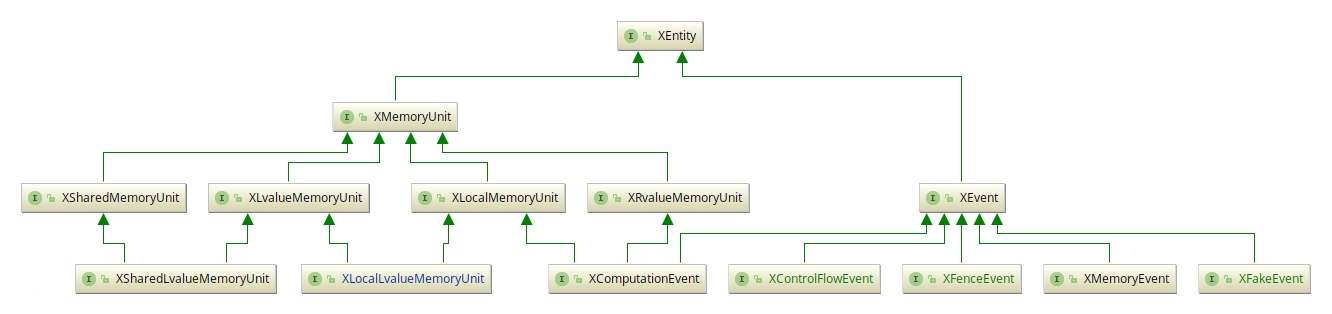
\includegraphics[width=\textwidth,keepaspectratio]{img/my/class-diagrams/XEntity-interfaces.png}
  \caption{The inheritance tree of interfaces of \xgraph{}}
  \label{fig:class-diagrams:XEntity-interfaces}
\end{figure}

All elements of \xgraph{} implement the interface \texttt{XEntity}.
There are two main kinds of X-entity: \textit{events} that implement the \texttt{XEvent} interface, and \textit{memory-units} that implement the \texttt{XMemoryUnit} interface.


\paragraph{Memory units}
\label{ch:impl:model:xgraph:mem}

The \textit{memory unit} is a memory cell of an abstract machine executing the code.
This machine has an infinite number of arbitrary-sized \textit{registers} (local memory units) and \textit{locations} (shared memory units).
Local memory units inherit the \texttt{XProcessLocalElement} interface, that stores the ID of the owning process.
Figure~\ref{fig:class-diagrams:XMemoryUnit} represents inheritance hierarchy of memory units.

\begin{figure}[t]%[!b]%[H]
  \centering
  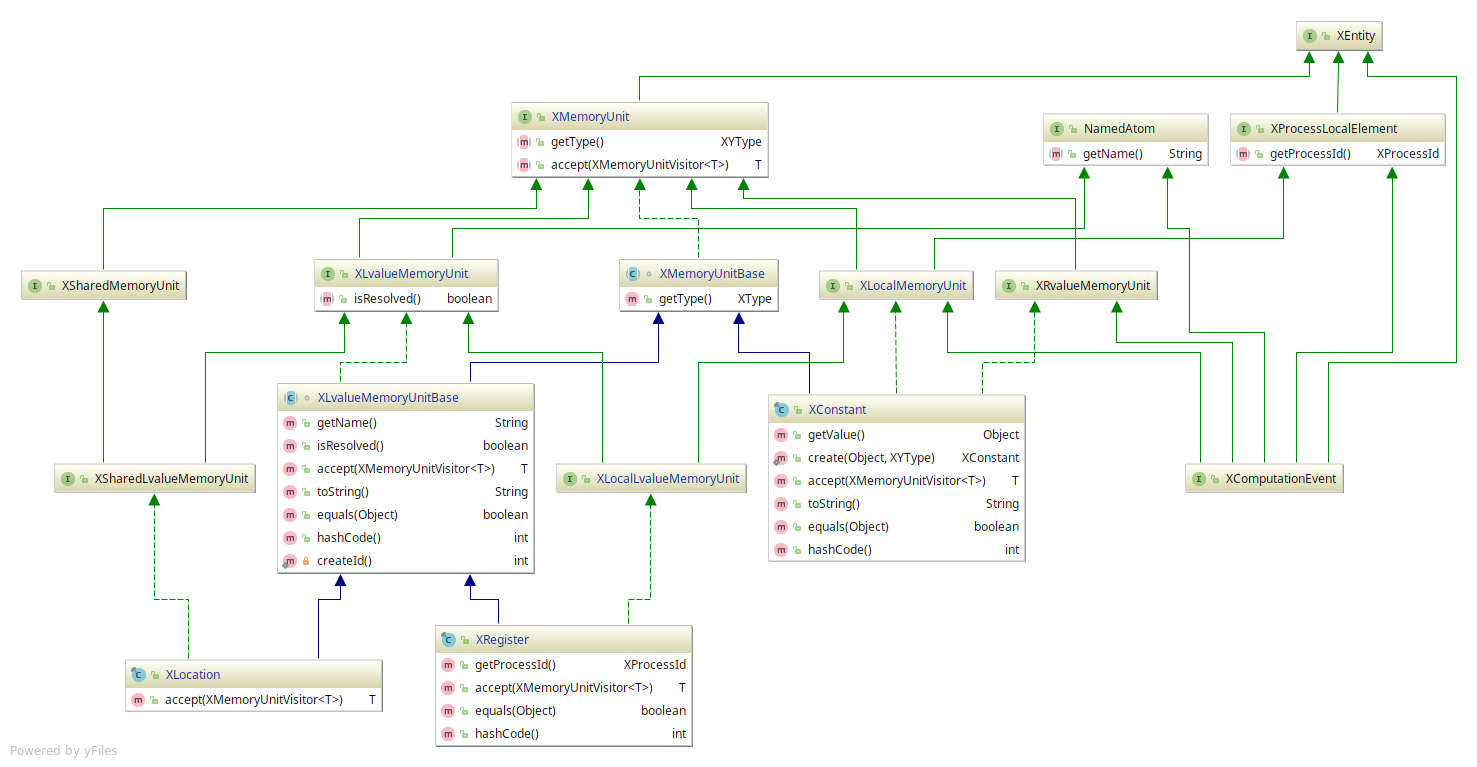
\includegraphics[width=\textwidth,height=\textheight,keepaspectratio]{img/my/class-diagrams/XMemoryUnit-m.png}
  \caption{The inheritance tree of \xgraph{} memory units}
  \label{fig:class-diagrams:XMemoryUnit}
\end{figure}

Following the terminology of the C standard, we distinguish the \textit{r-value} and \textit{l-value} memory units (unlike r-values, the l-values may be assigned a new value).
As r-values cannot change their value, they can be seen as the value itself (therefore the \texttt{XComputationEvent} is modelled as an local r-value memory unit, see more detailed discussion further in current Section).

Each memory unit has an \texttt{XType} associated with it.
The X-type is a symbolic representation of the C primitive type%
\footnote{Here we should note the \porthos[2] can eventually evolve to be able to analyse programs written in an OOP language (for instance, in C++). In this case, the \texttt{XType} will have more complex structure than a simple enumeration, which it has when we need to emulate only primitive types of C language. See more detailed discussion on input language type system in Section~\ref{ch:impl:proc:x-pre-compiler:type}.} %
that is easily convertable to a SMT type (modelled as \texttt{ZType}).%TODO: add the class ZType

- memory manager: no contexts so far; locals per process + shareds; register/deregister;


\paragraph{Events}
\label{ch:impl:model:xgraph:evt}

The following interfaces capture main types of events (see also Figure~\ref{fig:class-diagrams:XEntity-interfaces}):

\begin{itemize}
  \item \texttt{XMemoryEvent} \\
  The memory event defines the transfer of the value from one memory unit to another.
  There are four types of memory events (the arrow denotes the direction of the data-flow):
  \begin{enumerate}
  \item \texttt{XRegisterMemoryEvent}: \\
    $\texttt{XLocalLvalueMemoryUnit} \leftarrow \texttt{XLocalMemoryUnit}$
  \item \texttt{XLoadMemoryEvent}: \\
    $\texttt{XLocalLvalueMemoryUnit} \leftarrow \texttt{XSharedMemoryUnit}$
  \item \texttt{XStoreMemoryEvent}: \\
    $\texttt{XSharedLvalueMemoryUnit} \leftarrow \texttt{XLocalMemoryUnit}$
  \item \texttt{XInitialWriteEvent}: \\
    $\texttt{XLvalueMemoryUnit} \leftarrow \texttt{XRvalueMemoryUnit}$

  \end{enumerate}%TODO incompleted enumeration
  %TODO: either say st about getLoc(), getReg(), or remove them from code
  
  \item \texttt{XComputationEvent} \\
  - binary and unary \\
  - implements both \texttt{XEvent} and \texttt{XMemoryUnit}.
  This is a model-level optimisation possible \textbf{due to} because a computation-event
  %\textit{is} an event (thus it can form a node in \xgraph{}) and it also 
  performs a computation over local-only memory and does not change the value of any memory unit, therefore the \textit{computation} abstraction (the CPU time) can be safely removed from the model, and the computation event can be seen as an atomic operation.
  
  \item \texttt{XControlFlowEvent} \\
    \texttt{XJumpEvent} no computation, no data operation. may be safely removed for optimisation
    \texttt{XMethodCallEvent} : TODO: meth call should inherit both control-flow and computation.
    itself - computation result (temp register) + if (method resolved) => context binding + jump to the method body 
    
  \item \texttt{XFenceEvent}
    \texttt{XBarrierEvent} : mfence, sync, optsync, lwsync, optlwsync, ish, isb, isync
    
  \item \texttt{XFakeEvent}
    \begin{enumerate}
    \item \texttt{XEntryEvent}, the source event in the event-flow graph %only event that cannot have incoming edges
    \item \texttt{XExitEvent} : two kinds (depending on the unrolling boundary)
    \item \texttt{XNopEvent} : no-operation event, used for correct encoding (picture); same as simple jump to the next event
    \end{enumerate}
    
\end{itemize}

Edges (relations edges (just map with enum as kind of edge)):
\begin{enumerate}
\item CF edge: then-edge (primary), else-edge (alternative)
\item DF edge: co, rf
\end{enumerate}

Valid graph:
\begin{enumerate}
\item single source, two sinks
\item connected
\item each node has 1 or 2 children
\item branching node (2 children) instanceof XComputationEvent (evaluation of the value, no shared-memory operations)
\end{enumerate}

consider the following code in C:

picture of the CF-graph:

XEventInfo:
Events are specified by the process generated them and a unique label.
This information is stored by events as the immutable structure \texttt{XEventInfo}.
%hashcode, uniqueness

%\lstinputlisting{inc/XEventVisitor-cleaned.java}

\subsubsection{W-model}
\label{ch:impl:model:wmodel}
%TODO: almost not implemented !
<to be done>

a simple set of recursively defined relations over ..

atoms: sets/basic relations

itemize elements


\subsubsection{Z-formula}
\label{ch:impl:model:zformula}

%TODO: not implemented at all !

in \porthos[1] : ctx as an argument, calling ctx to create new clause. 
drawbacks:
- hard to debug
- only one solver
- non-safe way to construct formula (if ctx has changed, runtime excpetion)

in \porthos[2] we created the new abstraction layer \zformula that is translated to 

also recursive representation of smt formula

used as an abstrac

implemented as a simple wrapper over the z3 formula

typed: Expr, BoolExpr, ArithExpr, ...


\subsection{The processing units} %Transformation}
\label{ch:impl:proc}

%todo: after all, list HERE which modules (classes, managers) are being initialised during the pre-compilation. I'ts good to have the dependencies graph on moduls (operational semantics:) )

- numbers -- same as in gears in Figure~\ref{fig:arch}.

\subsubsection{Input memory model parser (1)}
\label{ch:impl:proc:inp-mod-parser}

ANTLR grammar is extracted from parser used by herd written in OCaml

\subsubsection{Input program parser (2)}
\label{ch:impl:proc:inp-prog-parser}
% todo: test pre-/post-fix operations //+think how current tool will behave if there's more than one post-operation //and pre-operation

%TODO: maybe merge this and previous subsubsections

todo: move something from the input language chapter here


\subsubsection{W-model constructor (3)}
\label{ch:impl:proc:w-constr}

visitor of antlr tree: almost direct

todo: grammar of w-model to appendix

in perspective: work with functional-style definitions

<not implemented yet>


\subsubsection{Y-tree constructor (4)}
\label{ch:impl:proc:y-constr}

from ANTLR syntax tree of C

- desugar, equiv transform

- variables distinguished from 

- if we don't support , our parser still parses it, and the error is thrown at the moment of converting syntax tree to the AST (Y-tree).

- So, The language-dependent syntax tree is converted to the AST by the stateless Visitor (e.g., for C11 -> Ytree conversion is made by 'C2YtreeConverterVisitor') + short structure of this visitor (how?.. need ly?)


\subsubsection{X-graph precompiler (5)}
\label{ch:impl:proc:x-pre-compiler}

%The original program encoded into the \texttt{XGraph} represents a \textit{flow graph}, a connected cyclic directed graph with single source node \texttt{(ENTRY)} (usually for convenience all leaves are connected to the sink node \texttt{(EXIT)}). The cycles are caused by low-level jump instructions, obtained from non-linear high-level control-flow statements (such as \texttt{while}, \texttt{do-while}, \texttt{for}, etc.). However, the cyclic flow graph cannot be encoded into SMT formula since ...
%//TODO:REFERENCE.%TODO

%note https://en.wikipedia.org/wiki/Semantics_(computer_science)
%Operational semantics loosely corresponds to interpretation,


\paragraph{The macro preprocessor}

typedefs, aliases

not supported yet

\paragraph{Variables kinds determination}
\label{ch:impl:proc:x-pre-compiler:var}

- pointers
- externs
- parameters of process-functions


\paragraph{The label resolution}
\label{ch:impl:proc:x-pre-compiler:label}

%TODO: <not implemented yet>

The label resolution is a process of linkage the referenced labels to declared labels.

In C, the labeled statements are declared via the colon-syntax `\texttt{<label> : <statement>}',
and the labels are referenced by the jump-statement `\texttt{goto <label>}'.
The label resolution algorithm traverses the \ytree{} and collects all declared labels into a map that points a label to the labeled statement. %TODO: code: remove temp label generation, it's stupid. put null.
This information is used during compilation (see Section~\ref{ch:impl:proc:x-compiler}).


\paragraph{Type analysis}% and function resolution.}
\label{ch:impl:proc:x-pre-compiler:type}

%TODO: remake this paragraph considering that we have already said sth about XType
The C language has a static (resolved at compile-time) manifest (all types are declared explicitly) type system.
Comparing to languages that use type inference, the type analysis of a C program constitutes a simple propagating the type information (obtained from variables declarations) to all expressions.
%In \porthos[2], the type is modelled by the class \texttt{XType}.%TODO: + fix class and package name!
Being carried at Y and X representation levels, the type is converted to a Z-type at the Z-formula encoding stage (see Section~\ref{ch:impl:proc:z-encoder}).

%TODO: describe the Type
%TODO: maybe rename back to XType
%TODO: but definitely get rid of bit32

- X-type construction: code of class YType2TypeConverter (todo: rename: it's not conversion, it's a type construction, from the y-level name+qualifiers+

- The typification algorithm: propagation rules for each of Y


\paragraph{Invocation hooking}
\label{ch:impl:proc:x-pre-compiler:hooks}

resolve the semantics of a function given its signature (meth name + params types)

knowledge base: InterceptionAction(BiFunction<XMemoryUnit, XMemoryUnit[], ? extends XEntity> action)


\subsubsection{X-graph compiler (6)}
\label{ch:impl:proc:x-compiler}

- hierarchy of Compilers (XCompiler is an stateful abstract machine)

Firstly, the \ytree{} is compiled to the \textit{cyclic control-flow event-based graph} \xgraph[CF].

Then: unrolled up to bound $k$ to the \textit{acyclic control-flow event-based graph} \xgraphU[CF].

Then: data-flow analysis to the \textit{acyclic full event-based graph} \xgraphU[CF+DF].

%MethCallE : bind parameters with values (load them to temp registers) + remember the return-register
%reutrn event= assign the return-register + simple jump


\subsubsection{X-graph unroller (7)}
\label{ch:impl:proc:x-unroll}

- unrolling: why we cannot encode cyclic structures. reference to the paper (see arXiv version)
% If the analysing program contains a loop, then its control-flow graph represents the cyclic directed graph. Although, in order to be able to encode such a cyclic structure as a boolean formula, this graph needs to be

simple algorithm

setting up backward edges

how we attempted, why it didn't work in general case:

why we changed the notion of unrolling bound

sth about hashcodes and collections

- After we acquired the event-based representation, we can perform some modifications/simplifications/optimisations on it (separately, allowing user to manage them)



%TODO: draw (and implement) diff types of exit nodes
\begin{figure}[h]
\centering
\resizebox{\linewidth}{!}{
\begin{tikzpicture}[->,>=stealth',shorten >=1pt,auto,node distance=1.5cm,semithick]
\node[c] (1) [] {$1$};
\node[c] (2) [below left of=1] {$2$};
\node[c] (3) [below right of=1] {$3$};
\node[c] (4) [below of=3] {$4$};
\path[->]
(1) edge [] node {} (2)
(2) edge [bend left=50,dotted] node {} (1)
(1) edge [] node {} (3)
(3) edge [] node {} (4)
(4) edge [bend right=80,dotted] node {} (1)
;
\node[draw=none] (impl) [right=3cm of 3] {$\overset{k = 6}{\longmapsto}$};
;
\node[c] (21) [right=3cm of impl] {$2_1$};
\node[c] (11) [above right=1cm and 1cm of 21]{$1_1$};
\node[c] (31) [below right=1cm and 1cm of 11] {$3_1$};
\node[c] (41) [below of=31] {$4_1$};
\node[c] (12) [below of=21] {$1_2$};
\node[c] (22) [below left=1cm and 1cm of 12] {$2_2$};
\node[c] (32) [below right=1cm and 1cm of 12] {$3_2$};
\node[c] (13) [below of=41] {$1_3$};
\node[c] (14) [below of=22] {$1_4$};
\node[c] (43) [below of=32] {$4_3$};
\node[c] (23) [below of=13] {$2_3$};
\node[c] (33) [below of=13] {$3_3$};
\node[c] (24) [below left=1cm and 1cm of 14] {$2_4$};
\node[c] (34) [below right=1cm and 1cm of 14] {$3_4$};
\node[c] (15) [below right=1cm and -0.3cm of 43] {$1_5$};
\node[c] (44) [below of=33] {$4_4$};
\node[c] (6) [below left=1cm and 1cm of 15] {$6$};
\node[] (11k) [right=3.2cm of 11] {$(k = 1)$};
\node[] (31k) [right=1.7cm of 31] {$(k = 2)$};
\node[] (41k) [right=1.7cm of 41] {$(k = 3)$};
\node[] (13k) [right=1.7cm of 13] {$(k = 4)$};
\node[] (33k) [right=1.7cm of 33] {$(k = 5)$};
\node[] (44k) [right=1.7cm of 44] {$(k = 6)$};
\path[->]
(11) edge [] node {} (21)
(11) edge [] node {} (31)
(31) edge [] node {} (41)
(21) edge [] node {} (12)
(12) edge [bend right=10] node {} (22)
(12) edge [bend left=10] node {} (32)
(41) edge [] node {} (13)
(22) edge [] node {} (14)
(32) edge [] node {} (43)
(13) edge [] node {} (23)
(13) edge [] node {} (33)
(14) edge [bend right=10] node {} (24)
(14) edge [bend left=10] node {} (34)
(43) edge [] node {} (15)
(33) edge [bend right=10] node {} (15)
(33) edge [bend left=10] node {} (44)
(24) edge [bend right=20] node {} (6)
(34) edge [] node {} (6)
(15) edge [] node {} (6)
(44) edge [bend left=20] node {} (6)
;
\end{tikzpicture}
}
\label{fig:loop-unwind}
\caption{Example of the flow graph from Figure~\ref{fig:merged-loop.....}, unwinded up to the bound $k = 6$}
\end{figure}


\subsubsection{X-graph data-flow constructor (8)}
\label{ch:impl:proc:x-df}%TODO: ref it in pre-word in this chapter

- set up co, rf edges => new graph

- computing SSA maps (now: during the encoding. should be: during the post-compilation) (as one of necessary steps before encoding)


\subsubsection{Z-formula encoder (9)}
\label{ch:impl:proc:z-encoder}

Z-type : SMT-specific (say about smt-lib)


\subsubsection{SMT-formula translator (10)}
\label{ch:impl:proc:smt-transator}%TODO: ref in pre-word


\subsubsection{SMT-formula translator (11)}
\label{ch:impl:proc:smt-solver}%TODO: ref it in pre-word in this chapter
%TODO: check that we have ALL references in pre-word in this chapter

%todo: mention The SMT-LIB standard http://smtlib.cs.uiowa.edu/papers/smt-lib-reference-v2.6-r2017-07-18.pdf


\subsection{Program output}
\label{ch:impl:out}

structure: verdict

%TODO: say sth about syntax errors handling: still now, what if parser does not accept syntax?



\subsection{Auxiliary components}
\label{ch:impl:aux}

\subsubsection{Watchdog timer}
\label{ch:impl:aux:watchdog}

<not implemented>

todo

\subsubsection{Logger}
\label{ch:impl:aux:logger}

<not implemented>

todo


%todo: some words on necessity of contexts and lack of them. How would we implement them

%todo: rename Interpreter -> Compiler.


%TODO: \section{Optimisations}